
% % \section{Rossby-Wellen}
% \begin{frame}{Rossby-Wellen auf der Kugel}
%     \begin{columns}
%       \column{0.55\textwidth}
%       \begin{itemize}
%         \item Idealisierte Strömung basierend auf der \textbf{Stromfunktion}:
%         \[
%           \psi(\theta, \phi) = \hat{\psi} \cos(k \phi) \sin(\theta)
%         \]
%         \item Daraus ergibt sich das Geschwindigkeitsfeld über:
%         \[
%           u = -\frac{1}{a} \frac{\partial \psi}{\partial \theta}, \quad
%           v = \frac{1}{a \sin \theta} \frac{\partial \psi}{\partial \phi}
%         \]
%         \item Wellenzahl \( k \), mittlerer Wind \( U_0 \), \\
%               Erdradius \( a \), Beta-Effekt implizit enthalten
%         \item Die Westwärts-Drift ist charakteristisch für Rossby-Wellen
%       \end{itemize}

%       \column{0.45\textwidth}
%       \centering
%       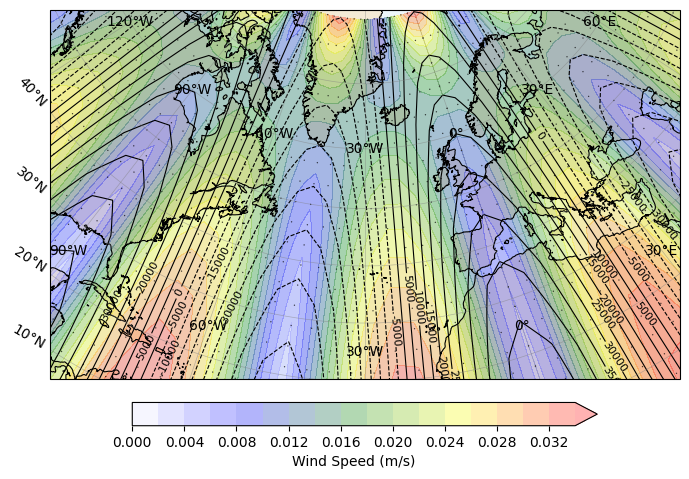
\includegraphics[width=\linewidth]{../images/rossby_wave_plot.png}
%     \end{columns}
%   \end{frame}

%   \begin{frame}{Rossby-Wellen auf der  $\beta$-Ebene}
%     \begin{columns}
%       \column{0.55\textwidth}
%       \begin{itemize}
%         \item Lineare Lösung der barotropen Vorticity-Gleichung auf der $\beta$-Ebene:
%         \[
%           \frac{\partial}{\partial t} \left( \nabla^2 \psi \right) + \beta \frac{\partial \psi}{\partial x} = 0
%         \]
%         \item Wellenansatz für die Stromfunktion:
%         \[
%           \psi(x, y, t) = \hat{\psi} \cos(kx + ly - \omega t)
%         \]
%         \item Dispersionsrelation:
%         \[
%           \omega = -\beta \frac{k}{k^2 + l^2}
%         \]
%         \item Geschwindigkeit:
%         \[
%           u = -\frac{\partial \psi}{\partial y}, \quad
%           v = \frac{\partial \psi}{\partial x}
%         \]
%         \item Charakteristisch: westwärts laufende Phasengeschwindigkeit bei \( \beta > 0 \)
%       \end{itemize}

%       \column{0.45\textwidth}
%       \centering
%       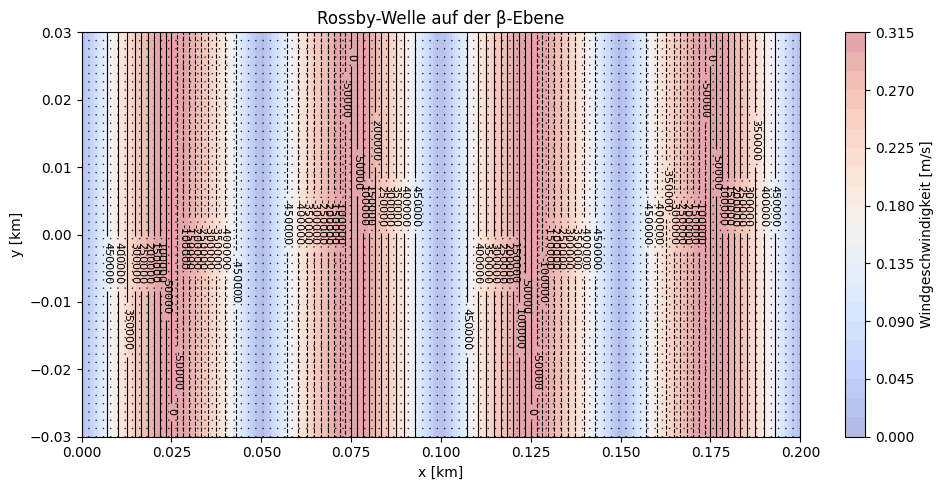
\includegraphics[width=\linewidth]{../images/rossby_wave_beta.png}
%       \scriptsize Darstellung: Windvektoren (Pfeile), Stromfunktion (schwarz), Windgeschwindigkeit (Farbflächen)
%     \end{columns}
%   \end{frame}


\begin{frame}{Rossby-Wellen}
	\begin{itemize}
		\item In Äquatornähe dominiert eine mittlere Ost-West-Strömung \( U \)
		\item Wir betrachten kleine Abweichungen davon:
		      \[
			      u' = U + u, \qquad v' = v \qquad \text{mit } u, v \ll U
		      \]
		\item Die Strömung ist quellenfrei → Stromfunktion \( \psi \) existiert:
		      \[
			      u = -\frac{\partial \psi}{\partial y}, \qquad v = \frac{\partial \psi}{\partial x}
		      \]
	\end{itemize}
\end{frame}

\begin{frame}{Zirkulation und Drehimpuls}
	\begin{itemize}
		\item Relative Vorticity (Zirkulation):
		      \[
			      \zeta = \frac{\partial v}{\partial x} - \frac{\partial u}{\partial y} = \Delta \psi
		      \]
		\item Absolute Vorticity:
		      \[
			      \zeta + f \qquad \text{(mit Coriolisparameter } f = f(y) \text{)}
		      \]
		\item Annahme: Erhaltung der absoluten Vorticity:
		      \[
			      \frac{d}{dt} (\zeta + f) = 0
		      \]
	\end{itemize}
\end{frame}

\begin{frame}{Bewegungsgleichung - Herleitung}
	\begin{itemize}
		\item Kettenregel für totale Ableitung:
		      \[
			      \frac{d}{dt} (\zeta + f)
			      =
			      \frac{\partial \zeta}{\partial t}
			      + (U+u) \frac{\partial \zeta}{\partial x}
			      + v \left( \frac{\partial \zeta}{\partial y} + \frac{\partial f}{\partial y} \right)
		      \]
		\item Näherungen:
		      \begin{itemize}
			      \item \( u \ll U \) → vernachlässigbar
			      \item \( \partial \zeta / \partial y \ll \partial f / \partial y \)
			      \item \( \partial f / \partial y = \beta \)
			      \item \( v = \frac{\partial \psi}{\partial x} \)
		      \end{itemize}
		\item Daraus ergibt sich:
		      \[
			      \frac{\partial \zeta}{\partial t}
			      + U \frac{\partial \zeta}{\partial x}
			      + \beta \frac{\partial \psi}{\partial x} = 0
		      \]
		\item Mit \( \zeta = \Delta \psi \):
		      \[
			      \frac{\partial \Delta \psi}{\partial t}
			      + U \frac{\partial \Delta \psi}{\partial x}
			      + \beta \frac{\partial \psi}{\partial x} = 0
		      \]
	\end{itemize}
\end{frame}

\begin{frame}{Wellenlösung der Gleichung}
	\begin{itemize}
		\item Ansatz: ebene Wellen
		      \[
			      \psi(x, y, t) = \cos(kx + ly - \omega t)
		      \]
		\item Einsetzen in Gleichung ergibt Dispersionsrelation:
		      \[
			      \omega = Uk - \frac{\beta k}{k^2 + l^2}
		      \]
		\item Phasengeschwindigkeit:
		      \[
			      c = \frac{\omega}{k} = U - \frac{\beta}{k^2 + l^2}
		      \]
		\item Interpretation: westwärts laufende Wellen mit geringer Geschwindigkeit als \( U \)
	\end{itemize}
\end{frame}

% \begin{frame}{Physikalisches Feld am Beispiel der Vorticity}
%   \begin{itemize}
%       \item Die \textbf{Vorticity} \( \zeta(x, y, t) \) beschreibt die Rotation eines Luftpakets.
      
%       \item Sie ist ein \textbf{physikalisches Skalarfeld}, das jedem Punkt eine Wirbelstärke zuordnet:
%       \[
%           \zeta = \frac{\partial v}{\partial x} - \frac{\partial u}{\partial y}
%       \]
      
%       \item In der Atmosphäre entsteht Vorticity durch:
%       \begin{itemize}
%           \item Wind-Scherung (Änderung der Windrichtung oder -geschwindigkeit)
%           \item Bewegung entlang der Breitenkreise (\( \beta \)-Effekt)
%       \end{itemize}
      
%       \item Die \textbf{Vorticity-Gleichung} beschreibt, wie sich dieses Feld entwickelt:
%       \[
%           \frac{\partial \zeta}{\partial t} + \vec{v} \cdot \nabla \zeta + \beta v = 0
%       \]
      
%       \item → Diese Gleichung ist eine typische \textbf{Feldgleichung}, weil sie die Änderung eines Feldes durch lokale und advektive Prozesse beschreibt.
%   \end{itemize}
%   \end{frame}
  